\documentclass[../main.tex]{subfiles}

\begin{document}

Considerando las necesidades de la red del segundo piso, y reconociendo las distintas áreas de trabajo, se identificaron tres subredes pertinentes para su cableado. Hay que notar que aunque nuestros switches tienen capacidades para más nodos, estas se mantendrán latentes para posibles expansiones en la red si llegan a ser necesarias, y solo se considerarán los 80 nodos planteados inicialmente.
\begin{itemize}
\item Geografía Física:
  Es la zona por mucho más grande, y por ende la que requiere más soporte de equipos. A esta subred le asignaremos una capacidad de 40 nodos.
\item LAGE:\@
  Identificamos las necesidades de esta zona, y decidimos asignarle 22 nodos.
\item Área Administrativa (Zona conjunta Dirección y Secretaría Administrativa):
  Consideramos que por su cercanía física y de necesidades, una sola subred puede cubrir ambas. A esta subred le asignaremos 18 nodos.
\end{itemize}

Ahora que definimos las necesidades de nuestras subredes, realizaremos las divisiones de las IP.\@ Consideraremos nuestra IP base a 177.164.4.0.

\subsubsection*{Geografía Física}
A esta la conoceremos como la subred 0. Ya que decidimos asignarle 40 nodos, requeriremos un número de nodos posibles potencia de dos. Por lo tanto esta red tendrá $2^6 - 2 = 62$ hosts. 
\\\\
Empezaremos la descripción de la subred:
\begin{itemize}
\item Máscara modificada: 255.255.255.192 o /26
\item Segmento: 177.164.4.0
\item Direcciones asignables: 177.164.4.1 -- 177.164.4.62
\item Broadcast: 177.164.4.63
\end{itemize}
\subsubsection*{LAGE}
A esta la conoceremos como la subred 1. Ya que decidimos asignarle 22 nodos, requeriremos un número de nodos posibles potencia de dos. Por lo tanto esta red tendrá $2^5 - 2 = 30$ hosts. 
\begin{itemize}
\item Máscara modificada: 255.255.255.224 o /27
\item Segmento: 177.164.4.64
\item Direcciones asignables: 177.164.4.65 -- 177.164.4.94
\item Broadcast: 177.164.4.95
\end{itemize}
\subsubsection*{Área Administrativa}
A esta la conoceremos como la subred 2. Ya que decidimos asignarle 18 nodos, requeriremos un número de nodos posibles potencia de dos. Por lo tanto esta red tendrá $2^5 - 2 = 30$ hosts. 
\begin{itemize}
\item Máscara modificada: 255.255.255.224 o /27
\item Segmento: 177.164.4.96
\item Direcciones asignables: 177.164.4.97 -- 177.164.4.126
\item Broadcast: 177.164.4.127
\end{itemize}
En este caso no requerimos subredes de enlace ya que la conectividad entre las subredes es dentro del mismo router.

Una vez configurada la red en PacketTracer para su prueba, se puede ver así:
\begin{figure}[H]
  \centering
  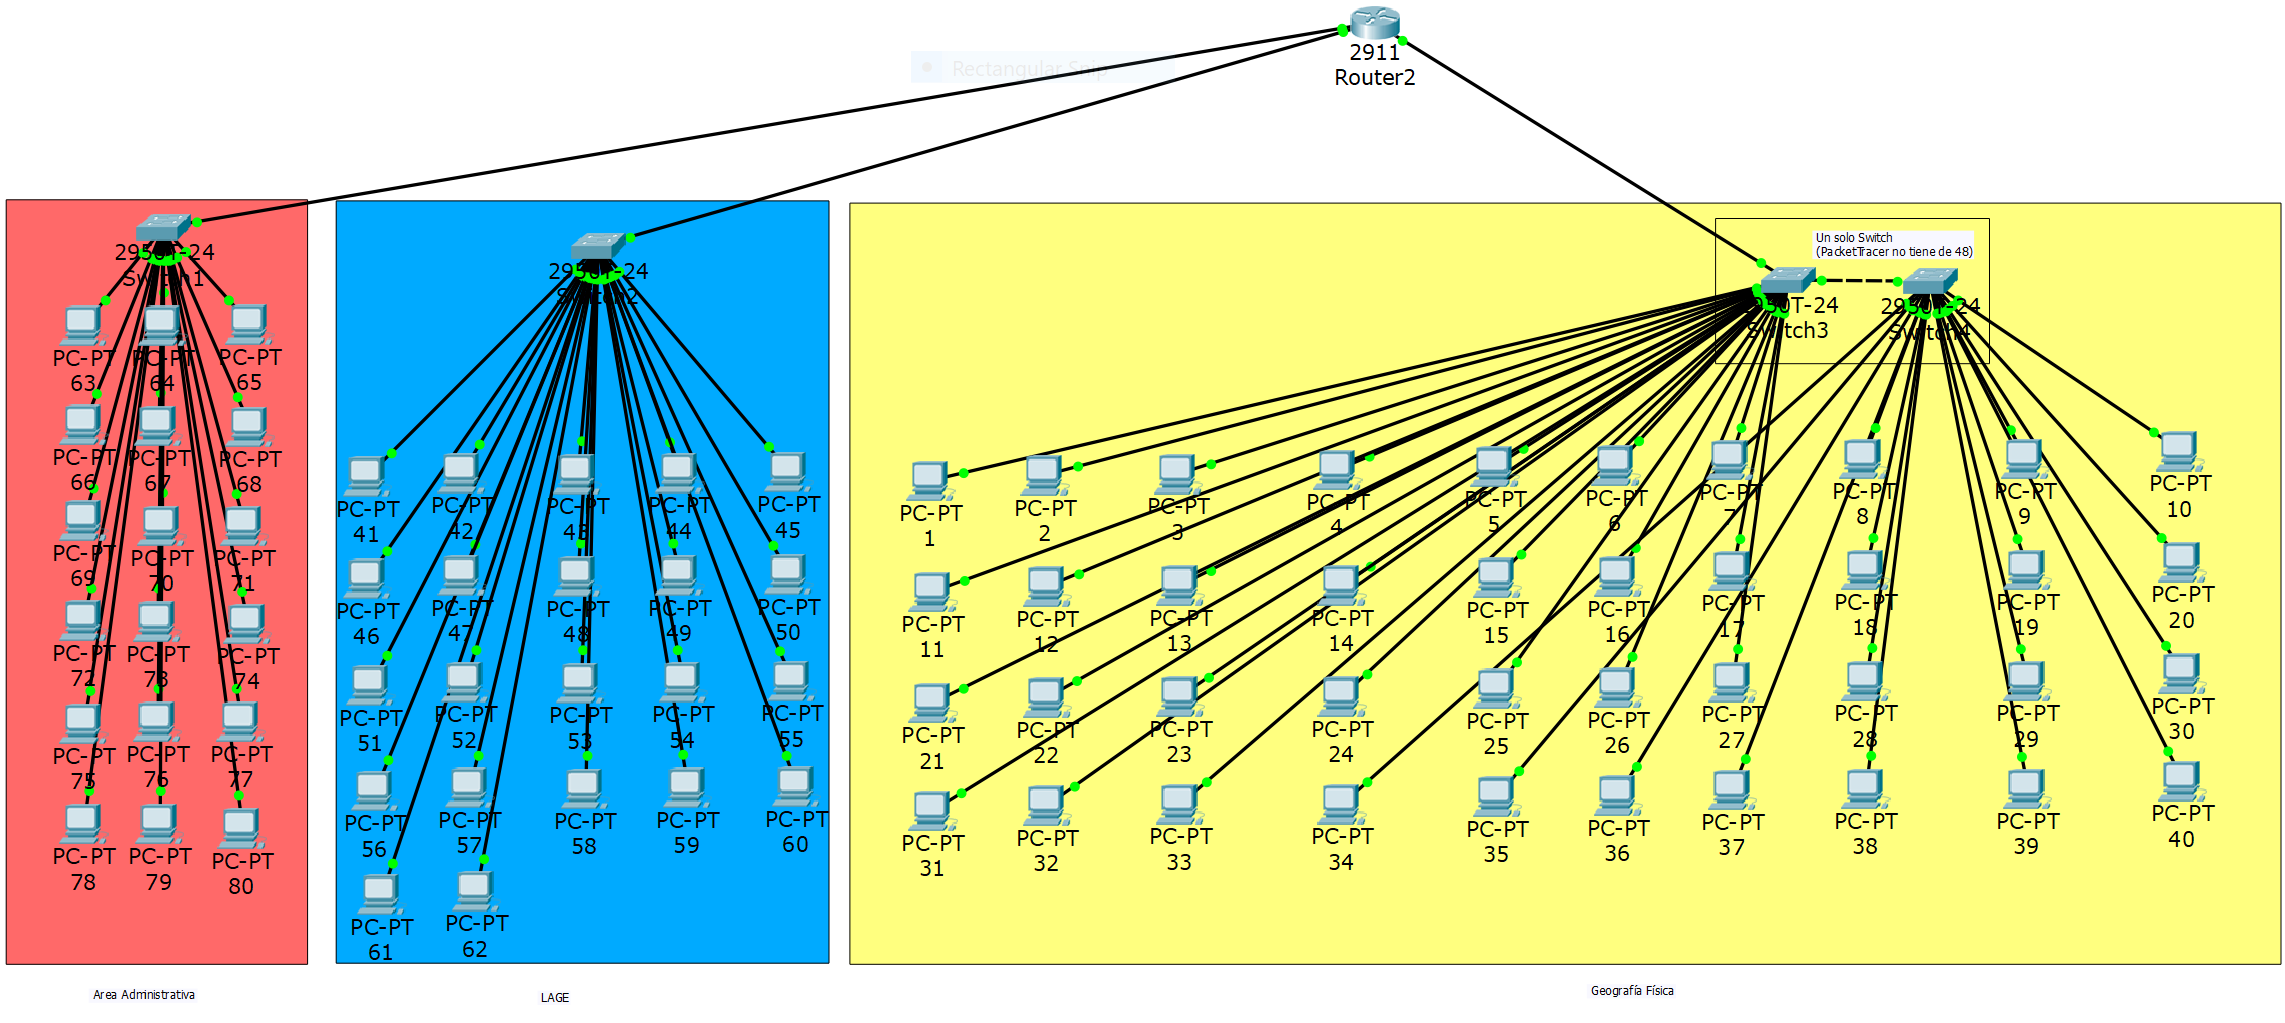
\includegraphics[width=\textwidth]{images/topologia.png}
  \caption{Topología de la red.}\label{fig:topo}
\end{figure}
Debe notarse que decidimos usar dos switches de 24 puertos y uno de 48 por los requerimientos de cada subred. Sin embargo, PacketTracer no tiene switches de 48 puertos incluidos, por lo que lo sustituimos por dos switches de 24 puertos en cascada. Esto en la práctica no sucedería porque procuraríamos tener el hardware necesario, pero fue necesario hacer esta sustitución para poder probar la configuración de la red. Los colores de los recuadros corresponden a la zona en la que se encuentran los equipos dado el siguiente diagrama:
\begin{figure}[H]
  \centering
  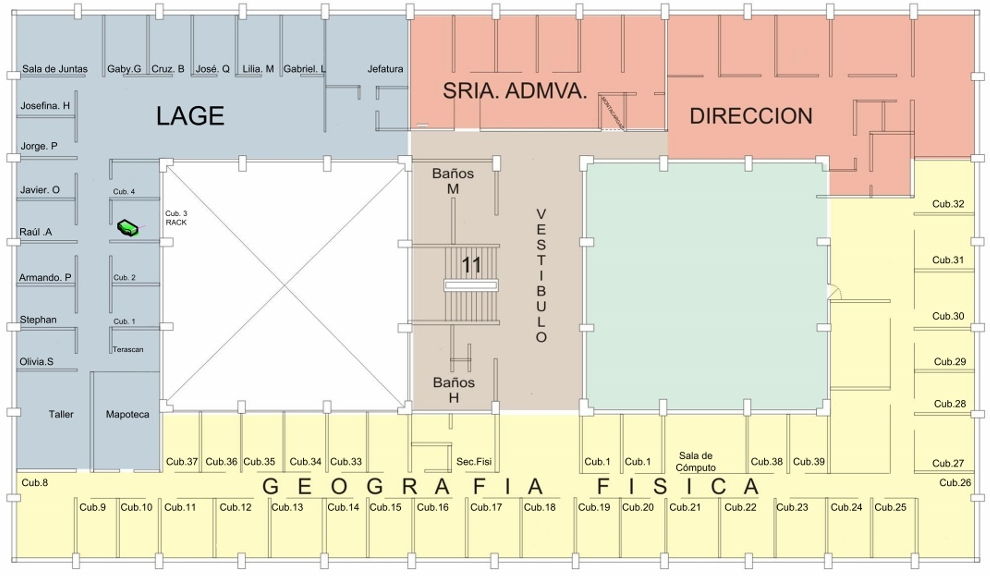
\includegraphics[width=\textwidth]{images/2p.jpg}
  \caption{Diagrama de las zonas del segundo piso.}\label{fig:topo}
\end{figure}
\subsection*{Configuración}
Para realizar la simulación, se tuvo que configurar el equipo de manera que se respetaran las subredes necesarias. A continuación daremos ejemplos de como se realizó la configuración para cada zona:
\subsubsection*{Geografía Física}

\begin{figure}[H]
  \centering
  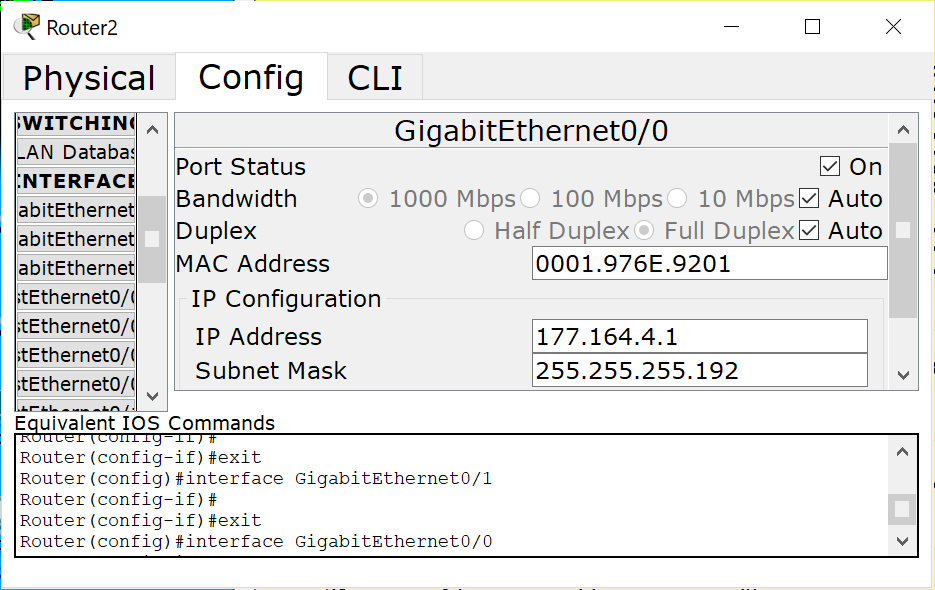
\includegraphics[width=0.4\textwidth]{images/1-port.PNG}
  \caption{Configuración del puerto del router para esta subred (dirección IP y máscara de subred)}\label{fig:ej11}
\end{figure}

\begin{figure}[H]
  \centering
  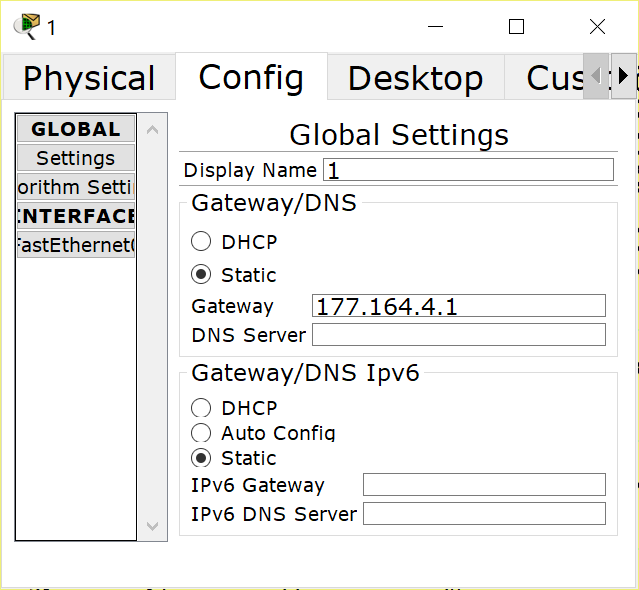
\includegraphics[width=0.4\textwidth]{images/1-g.PNG}
  \caption{Configuración de Gateway para un equipo de la subred}\label{fig:ej12}
\end{figure}

\begin{figure}[H]
  \centering
  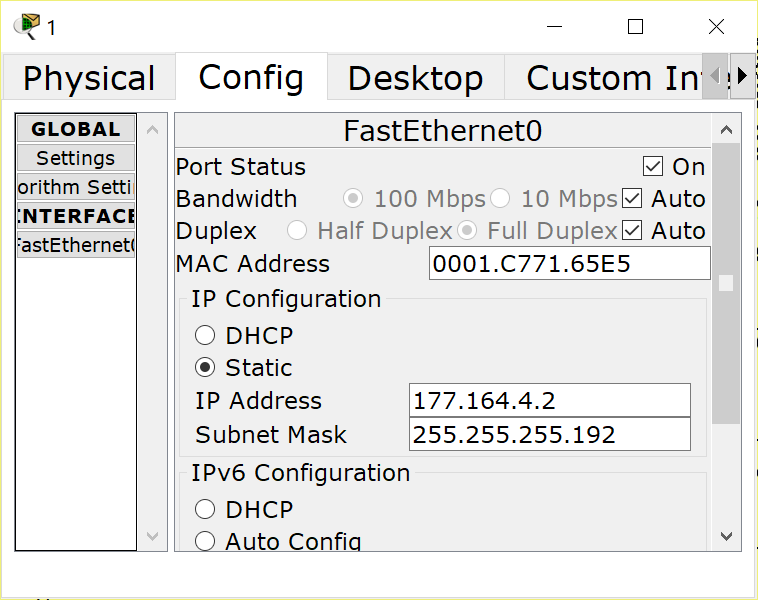
\includegraphics[width=0.4\textwidth]{images/1-ip.PNG}
  \caption{Configuración de dirección IP y máscara de subred para un equipo de la subred}\label{fig:ej13}
\end{figure}


\subsubsection*{LAGE}

\begin{figure}[H]
  \centering
  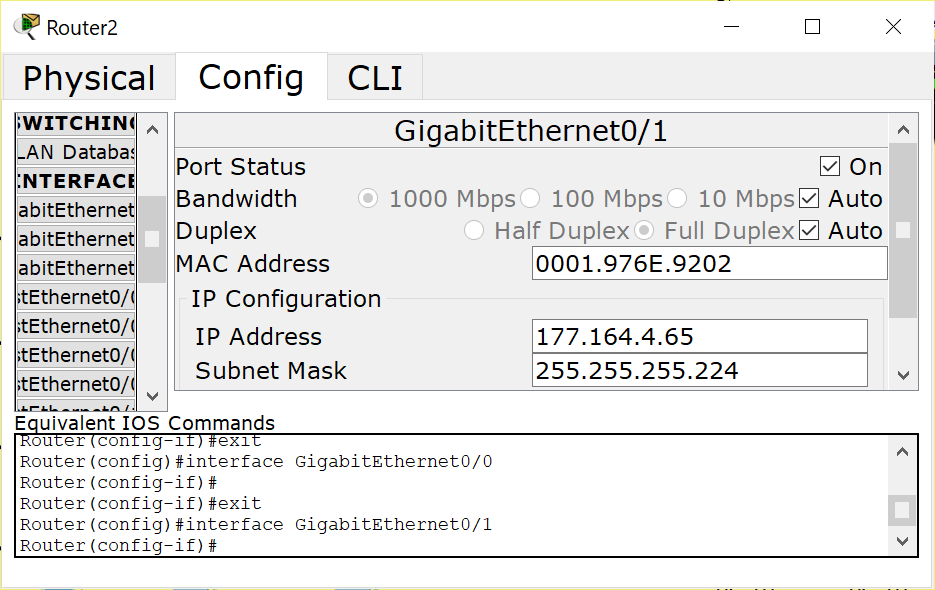
\includegraphics[width=0.4\textwidth]{images/2-port.PNG}
  \caption{Configuración del puerto del router para esta subred (dirección IP y máscara de subred)}\label{fig:ej21}
\end{figure}

\begin{figure}[H]
  \centering
  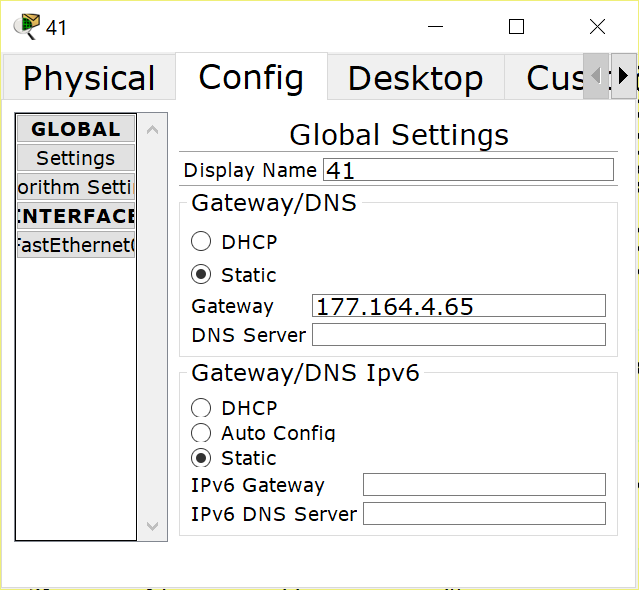
\includegraphics[width=0.4\textwidth]{images/2-g.PNG}
  \caption{Configuración de Gateway para un equipo de la subred}\label{fig:ej22}
\end{figure}

\begin{figure}[H]
  \centering
  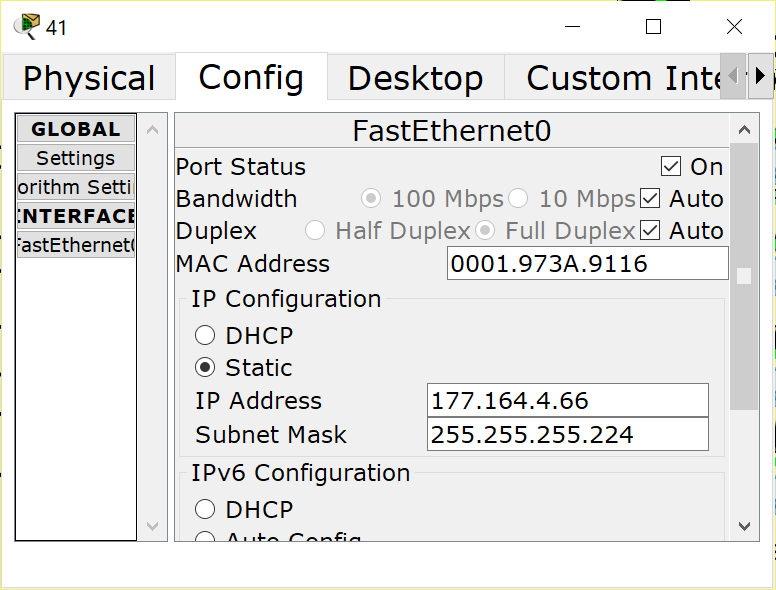
\includegraphics[width=0.4\textwidth]{images/2-ip.PNG}
  \caption{Configuración de dirección IP y máscara de subred para un equipo de la subred}\label{fig:ej23}
\end{figure}

\subsubsection*{Área Administrativa}

\begin{figure}[H]
  \centering
  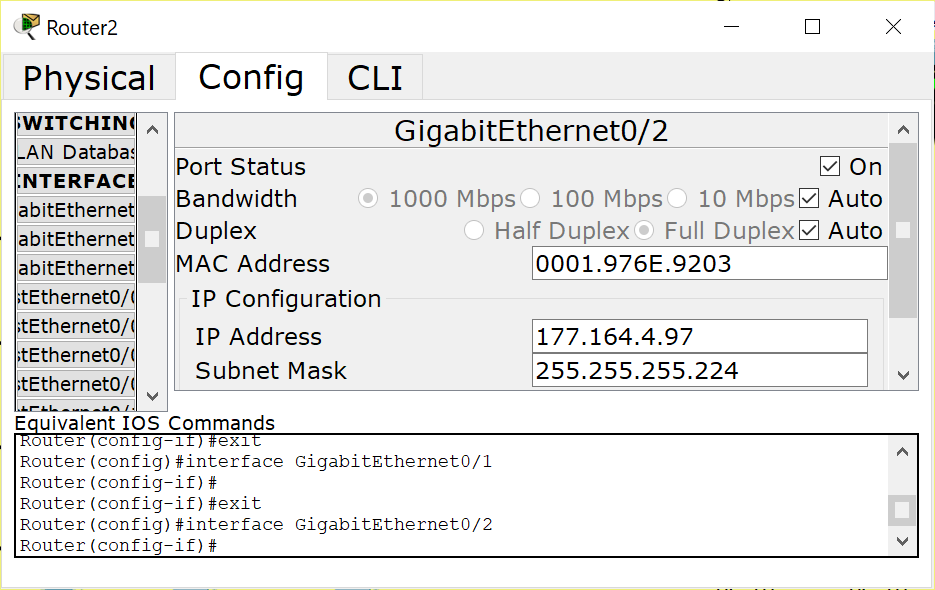
\includegraphics[width=0.4\textwidth]{images/3-port.PNG}
  \caption{Configuración del puerto del router para esta subred (dirección IP y máscara de subred)}\label{fig:ej31}
\end{figure}

\begin{figure}[H]
  \centering
  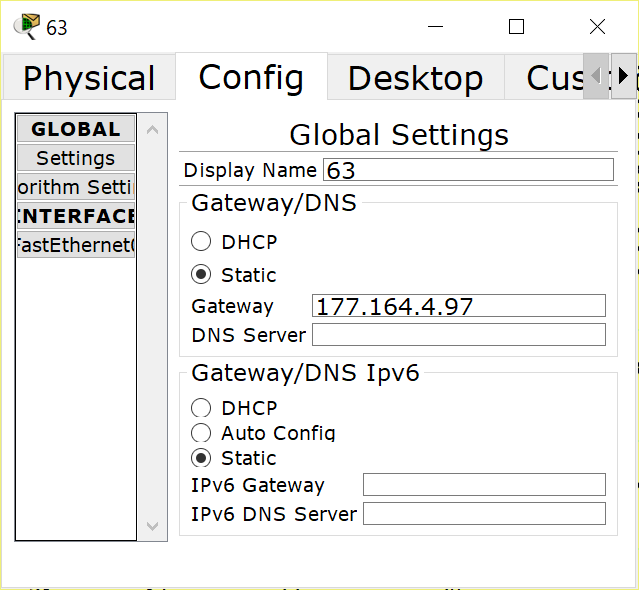
\includegraphics[width=0.4\textwidth]{images/3-g.PNG}
  \caption{Configuración de Gateway para un equipo de la subred}\label{fig:ej32}
\end{figure}

\begin{figure}[H]
  \centering
  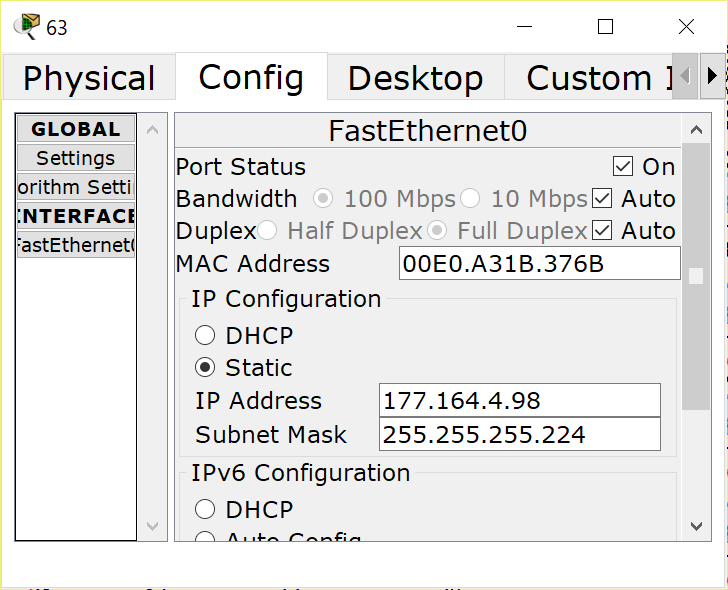
\includegraphics[width=0.4\textwidth]{images/3-ip.PNG}
  \caption{Configuración de dirección IP y máscara de subred para un equipo de la subred}\label{fig:ej33}
\end{figure}

\subsection*{Pruebas de conectividad}
Tras generar la red, se hicieron varias pruebas para demostrar la correcta configuración de las subredes. Como se podrá ver, se probaron todos los casos de conectividad dentro y fuera de las subredes.

\begin{figure}[H]
  \centering
  
\includegraphics[width=0.4\textwidth]{images/test1.PNG}
  \caption{Prueba de hacer un ping de un equipo en la subred 0 a otro en la subred 0.}\label{fig:t1}
\end{figure}

\begin{figure}[H]
  \centering
  
\includegraphics[width=0.4\textwidth]{images/test2.PNG}
  \caption{Prueba de hacer un ping de un equipo en la subred 0 a otro en la subred 1.}\label{fig:t2}
\end{figure}

\begin{figure}[H]
  \centering
  
\includegraphics[width=0.4\textwidth]{images/test3.PNG}
  \caption{Prueba de hacer un ping de un equipo en la subred 0 a otro en la subred 2.}\label{fig:t3}
\end{figure}

\begin{figure}[H]
  \centering
  
\includegraphics[width=0.4\textwidth]{images/test4.PNG}
  \caption{Prueba de hacer un ping de un equipo en la subred 1 a otro en la subred 1.}\label{fig:t4}
\end{figure}

\begin{figure}[H]
  \centering
  
\includegraphics[width=0.4\textwidth]{images/test5.PNG}
  \caption{Prueba de hacer un ping de un equipo en la subred 1 a otro en la subred 0.}\label{fig:t5}
\end{figure}

\begin{figure}[H]
  \centering
  
\includegraphics[width=0.4\textwidth]{images/test6.PNG}
  \caption{Prueba de hacer un ping de un equipo en la subred 1 a otro en la subred 2.}\label{fig:t6}
\end{figure}

\begin{figure}[H]
  \centering
  
\includegraphics[width=0.4\textwidth]{images/test7.PNG}
  \caption{Prueba de hacer un ping de un equipo en la subred 2 a otro en la subred 2.}\label{fig:t7}
\end{figure}

\begin{figure}[H]
  \centering
  
\includegraphics[width=0.4\textwidth]{images/test8.PNG}
  \caption{Prueba de hacer un ping de un equipo en la subred 2 a otro en la subred 0.}\label{fig:t8}
\end{figure}

\begin{figure}[H]
  \centering
  
\includegraphics[width=0.4\textwidth]{images/test9.PNG}
  \caption{Prueba de hacer un ping de un equipo en la subred 2 a otro en la subred 1.}\label{fig:t9}
\end{figure}

Como se puede notar, la configuración es correcta ya que es posible tanto generar comunicación en la misma subred, así como pasar esa comunicación al router que tiene puertos como Gateway de las otras subredes, lo que permite un correcto enrutamiento de la información. Si se deseara limitar estos accesos por políticas de acceso, podríamos recurrir a firewalls en el router para evitar la intercomunicación directa entre equipos de las distintas subredes.


\end{document}
